\documentclass{beamer}
\setbeamertemplate{navigation symbols}{}
\usepackage{comment}

\setbeamercolor{frametitle}{fg=black,bg=white}
\setbeamercolor{title}{fg=black,bg=yellow!85!orange}
\usetheme{AnnArbor}

\usepackage{textpos} % package for the positioning
\usepackage{listings}
\usepackage{xcolor}
\usepackage[most]{tcolorbox}
\usepackage{mathtools}
\usepackage{graphicx}
\usepackage{graphbox}
\usepackage{caption}
\DeclareCaptionType{code}[Code Listing][List of Code Listings] 

\definecolor{codegreen}{rgb}{0,0.6,0}
\definecolor{codegray}{rgb}{0.5,0.5,0.5}
\definecolor{codepurple}{rgb}{0.58,0,0.82}
\definecolor{backcolour}{rgb}{0.95,0.95,0.92} 
\lstdefinestyle{mystyle}{
    backgroundcolor=\color{backcolour},   
    commentstyle=\color{codegreen},
    keywordstyle=\color{magenta},
    numberstyle=\tiny\color{codegray},
    stringstyle=\color{codepurple},
    basicstyle=\ttfamily\footnotesize,
    breakatwhitespace=false,         
    breaklines=true,                 
    captionpos=b,                    
    keepspaces=true,                 
    numbers=left,                    
    numbersep=5pt,                  
    showspaces=false,                
    showstringspaces=false,
    showtabs=false,                  
    tabsize=2
}

\lstset{style=mystyle}

\lstdefinelanguage
   [x64]{Assembler}     % add a "x64" dialect of Assembler
   [x86masm]{Assembler} % based on the "x86masm" dialect
   % with these extra keywords:
   {morekeywords={CDQE,CQO,CMPSQ,CMPXCHG16B,JRCXZ,LODSQ,MOVSXD, %
                  POPFQ,PUSHFQ,SCASQ,STOSQ,IRETQ,RDTSCP,SWAPGS, %
                  rax,rdx,rcx,rbx,rsi,rdi,rsp,rbp, %
                  r8,r8d,r8w,r8b,r9,r9d,r9w,r9b, %
                  r10,r10d,r10w,r10b,r11,r11d,r11w,r11b, %
                  r12,r12d,r12w,r12b,r13,r13d,r13w,r13b, %
                  r14,r14d,r14w,r14b,r15,r15d,r15w,r15b}} %


\beamersetuncovermixins{\opaqueness<1>{25}}{\opaqueness<2->{15}}

%Copyright
\addtobeamertemplate{frametitle}{}{%
\begin{textblock*}{50mm}(0cm,-1.25cm)
\color{yellow!85!orange}
\tiny{Copyright \copyright 2024 CNM.}
\end{textblock*}}

% position the logo
\addtobeamertemplate{frametitle}{}{%
\begin{textblock*}{100mm}(11.4cm,-1.3cm)

\includegraphics[height=1cm,width=1cm,keepaspectratio]{fig/ddclogotransparent.png}
\end{textblock*}}

\AtBeginSection[]{
  \begin{frame}
  \vfill
  \centering
  \begin{beamercolorbox}[sep=8pt,center,shadow=true,rounded=true]{title}
    \usebeamerfont{title}\insertsectionhead\par%
  \end{beamercolorbox}
  \vfill
  \end{frame}
}

\begin{document}
\title{Quantum Math}
\author{Brian Rashap}
\date{August 2025} 



\begin{frame}
\titlepage
\end{frame}

\section{Algebra}
\begin{frame}\frametitle{Algebra Overview}
\begin{itemize}
\item Functions
\item Transformations
\item Polynomials
\item Rational Functions
\item Exponentials and Logarithms
\end{itemize}
\end{frame}

\begin{frame}\frametitle{Cartesian Coordinates}
\begin{columns}
\begin{column}{4cm}
Some text
\end{column}
\begin{column}{6cm}
\begin{center}
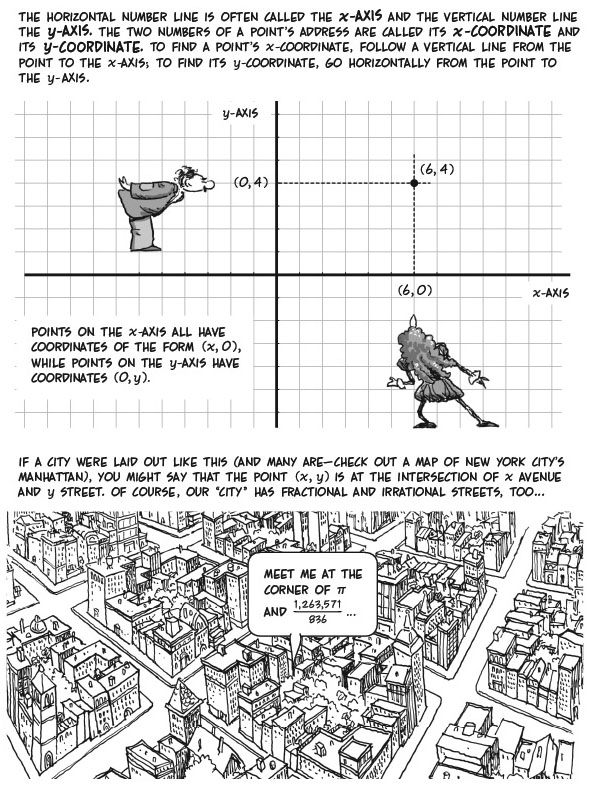
\includegraphics[height=7.5cm]{fig/plotting.jpg}
\end{center}
\end{column}
\end{columns}
\end{frame}

\begin{frame}\frametitle{Measuring Distance - Pythagorean Theorem}
\begin{columns}
\begin{column}{6cm}
Pythagorean Theorem:
\begin{center}
$a^2 + b^2 = c^2$
\end{center}

For example: \newline

\hspace*{10mm}$d^2 = 3^2 + 4^2$ \newline
\hspace*{10mm}$d^2 = 9 + 16 = 25$ \newline
\hspace*{10mm}$d = \sqrt{25} = 5$ \newline

More generally for two points $P(x_1,y_1)$ and $Q(x_2,y_2)$ \newline

\hspace*{10mm}$d^2 = (x_2-x_1)^2 + (y_2 - y_1)^2$ \newline
\hspace*{10mm}$d = \sqrt{(x_2-x_1)^2 + (y_2 - y_1)^2}$ \newline

Noting that $\mid a \mid = (a)^2$: \newline


\end{column}
\begin{column}{5cm}
\begin{center}
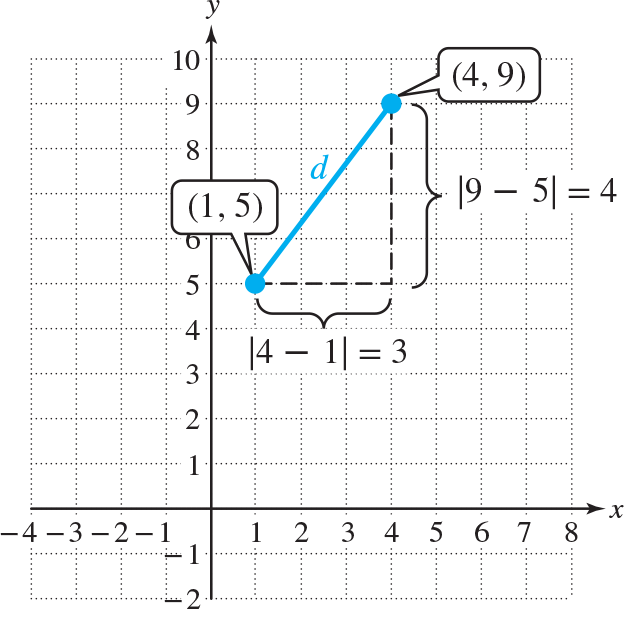
\includegraphics[width=4cm]{fig/pythag.png}
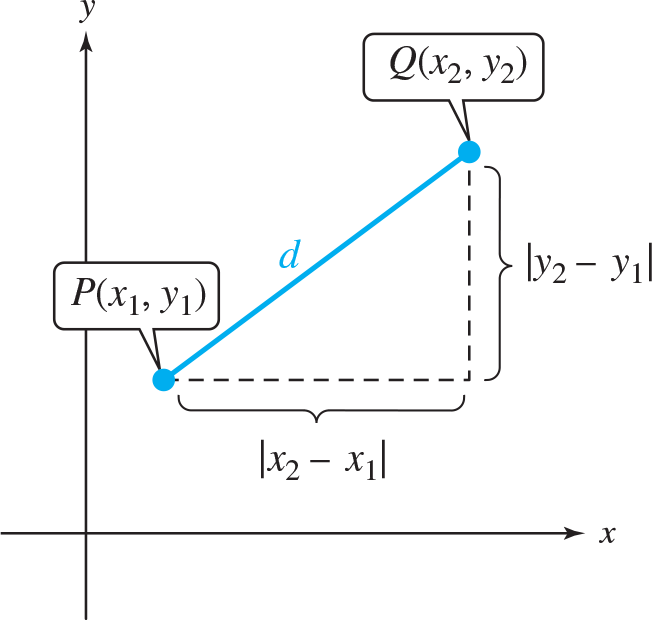
\includegraphics[width=4cm]{fig/pythag2.png}
\end{center}
\end{column}
\end{columns}
\end{frame}

\begin{frame}\frametitle{Midpoints and Intercepts}
\begin{columns}
\begin{column}{6cm}

Midpoint: \newline

\hspace*{10mm}$M = (\frac{x_1+x_2}{2},\frac{y_2+y_1}{2})$ \newline


Intercepts: \newline

Two key features of a graph are where the graph intersects the x and y axes, the x-intercept and y-intercept, respectively.


\end{column}
\begin{column}{5cm}
\begin{center}
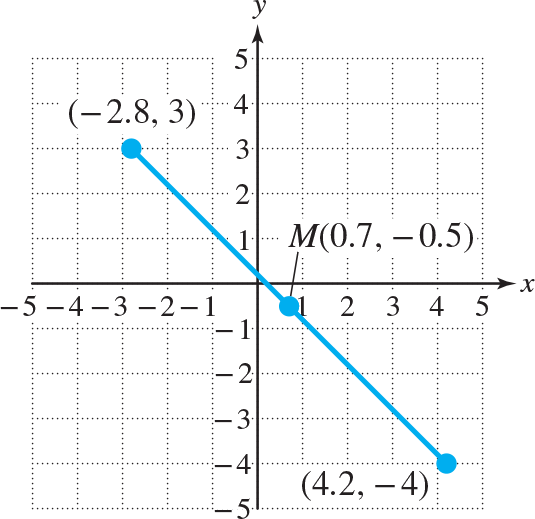
\includegraphics[width=4cm]{fig/midpoint.png}
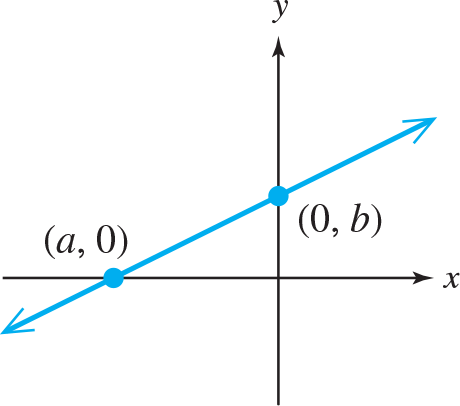
\includegraphics[width=4cm]{fig/intercept.png}
\end{center}
\end{column}
\end{columns}
\end{frame}


\begin{frame}\frametitle{The Circle}
\begin{columns}
\begin{column}{7.5cm}

A circle is a set of all points that are equidistant from a fixed point called the center $(h,k)$. The distance from any point on the cirecle to the center is called the radius ($r$)

$r = \sqrt{(x-h)^2 + (y-k)^2}$ \newline

Equation of a circle: \newline
Standard form: $(x-h)^2 + (y-k)^2 = r^2$ \newline

Expand binomials: $x^2-hx+h^2+y^2-ky+k^2 - r^2 = 0$ \newline

General form: $x^2+y^2-hx-ky+(h^2+k^2-r^2)=0$

\hspace*{10mm} or

$x^2 + y^2 + Ax + By + C = 0$

\end{column}
\begin{column}{3.5cm}
\begin{center}
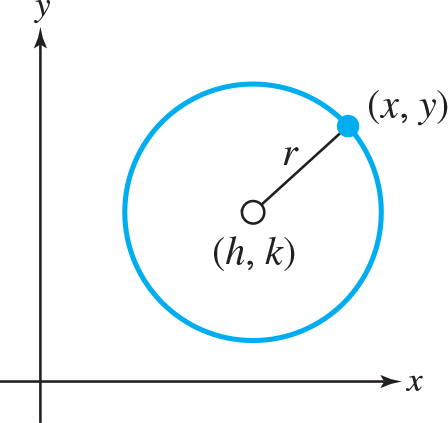
\includegraphics[width=3cm]{fig/circle.png}
\end{center}
\end{column}
\end{columns}
\end{frame}


\end{document}
